\documentclass[a4paper,11pt]{article}
\usepackage[framed,numbered]{matlab-prettifier}
\usepackage{caption}
\usepackage{graphicx}
\usepackage{subcaption}
\begin{document}
	\begin{titlepage}
		
		\newcommand{\HRule}{\rule{\linewidth}{0.5mm}} % Defines a new command for the horizontal lines, change thickness here
		
		\center % Center everything on the page
		
		
		
		\textsc{\LARGE Department of  }\\[0.3cm] % Name of your university/college
		\textsc{\LARGE Robotics and Mechatronics Engineering  }\\[0.3cm]
		\textsc{\Large   }\\[0.3cm]
		\textsc{\Large Lab report }\\[0.5cm] % Major heading such as 
		
		\HRule \\[0.4cm]
		{ \huge \bfseries DIGITAL SIGNAL PROCESSING}\\[0.4cm]  
		
		{ \huge \bfseries (CSE-401)}\\[0.03cm]
		% Title of your document
		\HRule \\[5cm]
		
		
		
		\begin{minipage}{0.4\textwidth}
			\begin{flushleft} \large
				\emph{Submitted By:}\\
				Md. Tahmeed Abdullah \\Roll: SH-092-002\\$4^{th}$ year $1^{st}$ semester % Your name
			\end{flushleft}
		\end{minipage}
		~
		\begin{minipage}{0.4\textwidth}
			\begin{flushright} \large
				\emph{Submitted To:} \\
				Mr. Sujan Sarker\\Lecturer\\Dept. of RME % Supervisor's Name
			\end{flushright}
		\end{minipage}\\[1cm]
		
		
		
		\vfill
			
		
		
	\end{titlepage}
	\begin{center}
		
	\end{center}
	\section*{Experiment no. 4}
	\section*{Name of the experiment}
	Using cross-correlation to find delay between input and output signals
	\section*{Objectives}
	\begin{itemize}
		\item To learn how to use linear filters. 
		\item To understand the basics of cross-correlation.
		\item To learn how radar and other distance sensors use correlation to find distance of objects
		
	\end{itemize}
	\section*{Theory}
	In general, correlation describes the mutual relationship which exists between two or more things. The same definition holds good even in the case of signals. That is, correlation between signals indicates the measure up to which the given signal resembles another signal. In other words, if we want to know how much similarity exists between the signals 1 and 2, then we need to find out the correlation of Signal 1 with respect to Signal 2 or vice versa.
	
	There are two types of Correlation in signal processing. These are:\\
	\begin{itemize}
		\item This is a kind of correlation, in which the signal in-hand is correlated with another signal so as to know how much resemblance exists between them. The cross-correlation of the discrete time signals x [n] and y [n] is expressed as
		$$ R_{xx}[m]= \sum_{n=-\infty}^{\infty}x[n]x[n-m] $$
		\item Auto Correlation is a type of correlation in which the given signal is correlated with itself, usually the time-shifted version of itself.
		The auto correlation of a discrete time signal x[n] is
		$$ R_{xy}[m]= \sum_{n=-\infty}^{\infty}x[n]y[n-m] $$
	\end{itemize}

	A signal is transmitted and received by a digital device. If there is no delay between the signals, the auto-correlation of the transmitted and received signal will have a peak at $n=0$, because the two signal are exactly equal to each other(if we neglect transmission losses), at $n=0$.
	
	If there is a delay between the two signals, the peak in the correlation signal will be shifted from the origin. The amount of shift determines the time delay between the two signals.
	
	\begin{figure}[h!]
		\centering
		\begin{subfigure}[h]{0.4\linewidth}
			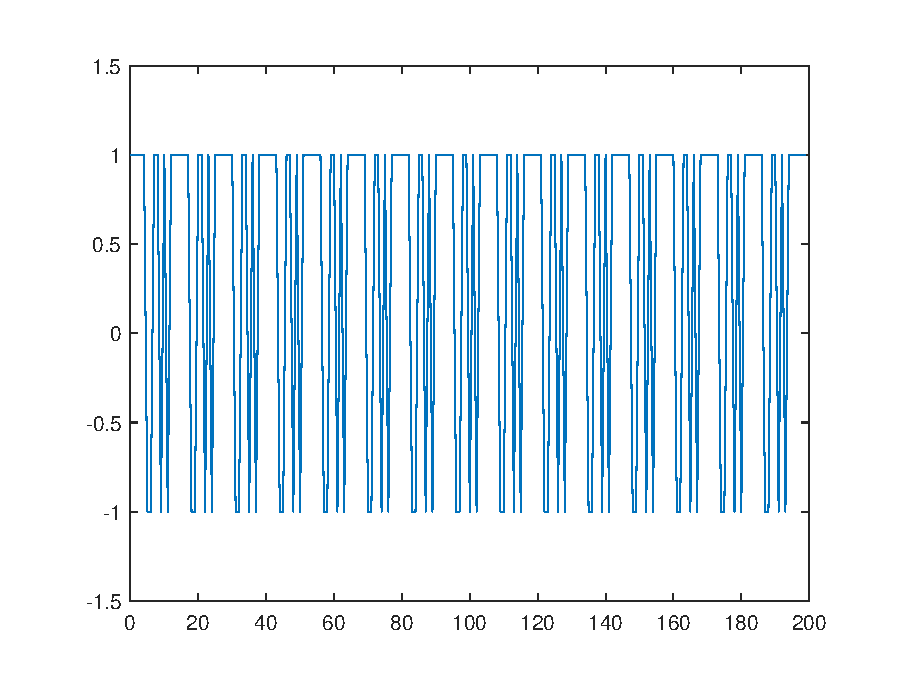
\includegraphics[width=\linewidth]{transmit.eps}
			\caption{Transmitted signal x[n]}
			\label{fig:transmitted_signal}
		\end{subfigure}
		\begin{subfigure}[h]{0.4\linewidth}
			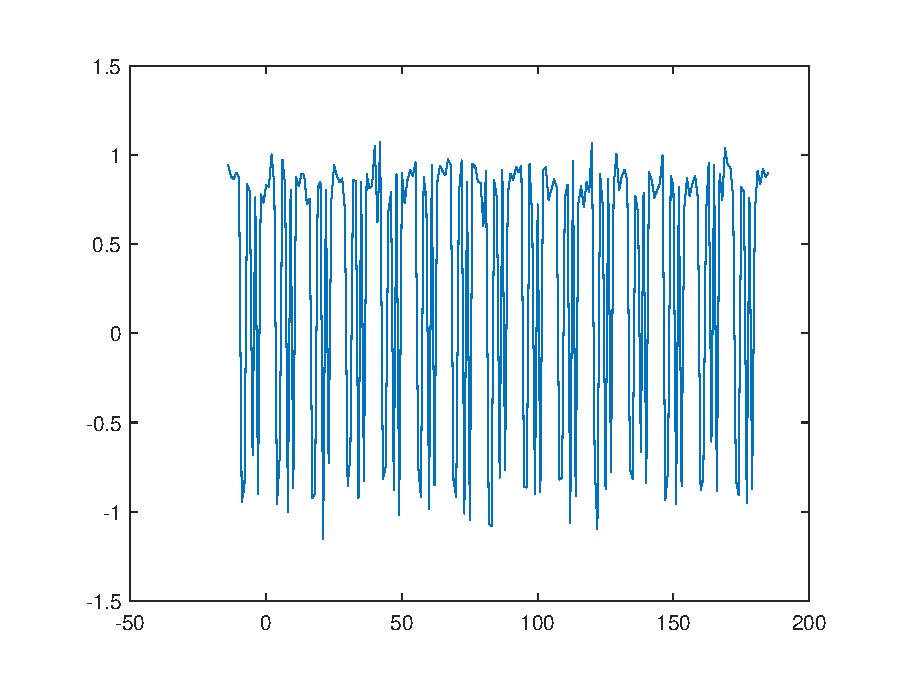
\includegraphics[width=\linewidth]{receive.eps}
			\caption{Received signal y[n]}
			\label{fig:received_signal}
		\end{subfigure}
		\caption{Transmitted and received signal}
	\end{figure}
	For a digital measuring device let x[n] be the transmitted signal and y[n] be the received signal where
	$$ y[n] = a \times x[n-D] + v $$ 
	In figure \ref{fig:transmitted_signal} we have a signal x[n] and in figure \ref{fig:received_signal} we have the received signal y[n]. The input signal is attenuated by factor $a$, delayed by $D$ samples and the noise induction in the signal is $v$.
	\begin{figure}[h!]
		\centering
		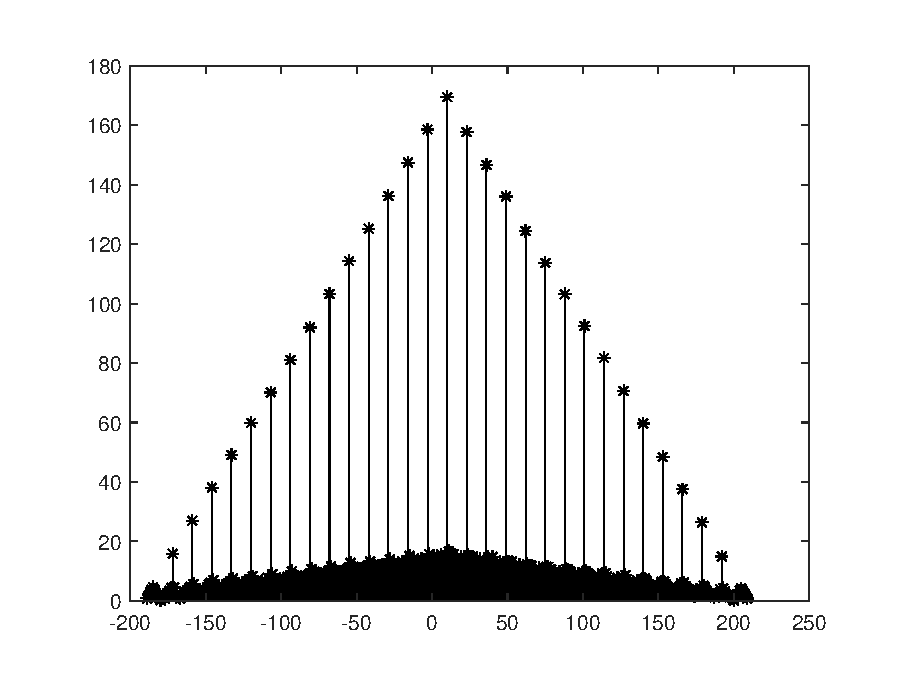
\includegraphics[scale=0.5]{rxy.eps}
		\caption{$R_{xy}$; Cross correlation of x \& y}
		\label{fig:rxy}
	\end{figure}
	
	If we calculate the cross correlation of the two signals we get the graph in figure \ref{fig:rxy}. If observed, the peak is shifted by some sample N which is the time delay between the two signals.
	
	\section*{Implementation Code}  
	\captionsetup{labelformat=empty,labelsep=none}
	\lstinputlisting[style = Matlab-editor, caption={main.m}]{../lab5.m}
	\vspace{1.5cm}
	\large Functions Used:
	
	\lstinputlisting[style = Matlab-editor, caption={ccor.m}]{../ccor.m}
	
	\lstinputlisting[style = Matlab-editor, caption={convolute.m}]{../convolute.m}
	\lstinputlisting[style = Matlab-editor, caption={shift.m}]{../shift.m}
	\lstinputlisting[style = Matlab-editor, caption={fold.m}]{../fold.m}
	
	
	
\end{document}